\documentclass{article}
\usepackage[utf8]{inputenc}
\usepackage[T1]{fontenc}
\usepackage[portuguese]{babel}

\usepackage{indentfirst}
\usepackage{makeidx}
\usepackage{stackengine}
\usepackage{amssymb}
\usepackage{amsthm}
\usepackage{hyperref}
\usepackage{color}
\usepackage{graphicx}


\title{\bf{Aprendizagem Computacional - Trabalho Prático 2}\vspace{80mm}}
\author{\textbf{João Tiago Márcia do Nascimento Fernandes - 2011162899} \\
\textbf{Joaquim Pedro Bento Gonçalves Pratas Leitão - 2011150072}}
\makeindex

\begin{document}

\maketitle

\pagebreak

\renewcommand*\contentsname{Índice}
\tableofcontents

\pagebreak

\section{Introdução}

Este trabalho foca-se no reconhecimento de caracteres da numeração árabe, ou seja, os caracteres 0 a 9.

Pretende-se que este reconhecimento seja realizado por uma aplicação desenvolvida em \emph{Matlab}, que faz uso de redes neuronais na sua arquitetura interna, disponíveis na \emph{Nerual Networks Toolbox} do próprio \emph{Matlab}.

A aplicação desenvolvida visa o estudo de duas arquiteturas distintas no reconhecimento dos caracteres:

\begin{itemize}
\item Na primeira arquitetura a aplicação será constituída por uma \emph{memória associativa} e um \emph{classificador}

\item Na segunda arquitetura a aplicação apenas recorre ao \emph{classificador}
\end{itemize}

\vspace{.3cm}

As duas arquiteturas apresentadas estão presentes nas figuras que se seguem:

\begin{figure}[h]
  \centering
      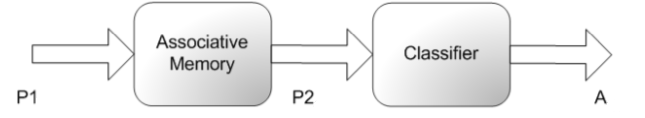
\includegraphics[scale=0.4]{AM_Classifier.png}
  \caption{Arquitetura da aplicação com \emph{memória associativa + classificador}}
\end{figure}

\begin{figure}[h]
  \centering
      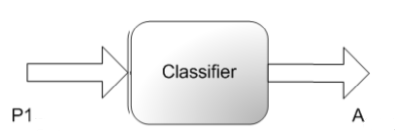
\includegraphics[scale=0.4]{Classifier.png}
  \caption{Arquitetura da aplicação apenas com o \emph{classificador}}
\end{figure}

Através da análise destas figuras podemos determinar um comportamento padrão para a aplicação:

\begin{itemize}
\item Numa fase inicial, os caracteres a identificar poderão, ou não, ser fornecidos à \emph{memória associativa}, que está encarregue da sua "filtragem" ou "correção": Se os caracteres fornecidos não forem perfeitos, a memória associativa aproxima-os dos respetivos caracteres perfeitos.

\item De seguida os dados, corrigidos ou não, serão fornecidos ao \emph{classificador}, que se encarregará de proceder à identificação dos mesmos.
\end{itemize}

No presente documento iremos proceder à apresentação em maior detalhe destas duas arquiteturas e das suas implementações, bem como da aplicação \emph{Matlab} desenvolvida, e de como poderá ser utilizada. Pretendemos também fazer uma análise crítica da performance da aplicação, nomeadamente da sua capacidade de classificar corretamente novos caracteres fornecidos.

\pagebreak

\section{Aplicação Desenvolvida}

A aplicação desenvolvida visa identificar corretamente caracteres desenhados pelo utilizador, implementando para isso as duas arquiteturas apresentadas anteriormente: \emph{Memória Associativa + Classificador} e \emph{Classificador}.

Ambas as arquiteturas e os respetivos modos de funcionamento serão apresentados de seguida.

\subsection{Memória Associativa + Classificador}

Na arquitetura \emph{Memória Associativa + Classificador}, os caracteres desenhados pelo utilizador, que constituem o \emph{input} da nossa aplicação, são fornecidos à \emph{memória associativa}, onde são \emph{"purificados"}.

Com esta operação pretende-se aproximar os caracteres desenhados pelo utilizador, que são naturalmente imperfeitos, dos respetivos caracteres perfeitamente desenhados. Ao purificarmos os dados estaríamos a aumentar a sua precisão, o que, teoricamente, resultará numa melhor classificação por parte do \emph{classificador}.

Por seu turno, o \emph{classificador} recebe como entradas os caracteres purificados e, com recurso a uma rede neuronal previamente treinada, processa cada uma das suas entradas, produzindo uma classificação para cada uma delas, que corresponde à identificação do caracter em questão, classificação essa que será apresentada ao utilizador.

\subsection{Classificador}

Ao contrário da arquitetura anterior, na arquitetura \emph{Memória Associativa + Classificador}, os caracteres desenhados pelo utilizador não sofrem qualquer tipo de purificação, sendo fornecidos ao \emph{classificador} tal como foram desenhados pelo utilizador.

Tal como o descrito na arquitetura anterior, o classificador recorre a uma rede neuronal previamente treinada para realizar a classificação das entradas. Uma vez classificadas as entradas, o resultado da sua classificação é apresentado ao utilizador.

\pagebreak

\subsection{Implementação em Matlab}

Para o desenvolvimento da aplicação foi-nos fornecido código-fonte, que cria e disponibiliza ao utilizador uma grelha onde este irá desenhar os caracteres a identificar, encarregando-se de toda a lógica interna da aplicação com a exceção da implementação do sistema de classificação dos caracteres e de toda a lógica a ele inerente (implementação das diferentes arquiteturas da aplicação, realização dos treinos das redes neuronais implementadas, etc)

\subsubsection{associativeMemory.m}

Neste ficheiro encontra-se uma pequena implementação da memória associativa, presente na função \emph{associativeMemory}. Esta implementção visa \emph{"purificar"} os caracteres desenhados pelo utilizador, aproximando-os do respetivo caracter perfeitamente desenhado. Nesta implementação apenas são calculados os pesos da rede neuronal que constituí a \emph{memória associativa}.

O cálculo dos pesos é feito de duas formas diferentes, dependendo do número de protótipos e de entradas fornecidos à \emph{memória associativa}, e recorrendo a um conjunto de dados de treino.

Assim, se o número de protótipos for superior ao número de entradas, os pesos são calculados de acordo com a fórmula: $target\times input^{T}\times \left(input\times input^{T}\right)^{-1}$, onde \emph{input} corresponde aos dados de treino fornecidos à \emph{memória associativa}, e \emph{target} corresponde aos respetivos valores esperados à saída da \emph{memória associativa}.

Caso contrário, ou seja, caso o número de protótipos seja igual ou inferior ao número de entradas, os pesos são calculados de acordo com a fórmula: $target\times pinv(input)$, onde \emph{input} e \emph{target} representam, respetivamente, os dados fornecidos à \emph{memória associativa} e os valores à saída.

Uma vez calculados os valores desses pesos a função \emph{associativeMemory} retorna, devolvendo os valores calculados. A \emph{"purificação"} dos dados criados pelo utilizador só será realizada na função \emph{myclassify} (presente no ficheiro \emph{myclassify}), após terem sido obtidos os pesos da \emph{memória associativa}.

\subsubsection{createNetwork.m}

No ficheiro \emph{createNetwork.m} encontramos a função \emph{createNetwork}, responsável pela criação e treino de uma rede neuronal que representará o \emph{classificador}.

Esta rede é criada de acordo com algumas características pré-definidas, e um conjunto de características escolhidas pelo utilizador, como é o caso da função de ativação. Uma vez criada a rede neuronal, esta é treinada com um conjunto de dados previamente obtidos, e que se encontram nos ficheiros \emph{PTreino500.mat} e \emph{Tfinal500.mat}.


\subsubsection{myclassify.m}

No ficheiro \emph{myclassify.m} encontramos a função \emph{myclassify}, onde se encontra uma boa parte da lógica principal da aplicação.

Esta função é chamada pela função \emph{ocr\_func}, que por sua vez é chamada pela função \emph{mpaper}, e recebe como argumento os caracteres desenhados pelo utilizador.

Caso o utilizador tenha indicado a utilização de uma \emph{memória associativa}, e qual o método para o cálculos dos seus pesos, a função verifica se a \emph{memória associativa} pretendida já foi previamente criada. Caso tenha sido criada, os seus pesos são carregados em memória e os caracteres desenhados pelo utilizador são \emph{"purificados"}. Caso nenhuma tenha sido criada, a \emph{memória associativa} é criada, os seus pesos são determinados com base em valores de treino previamente computados, e de seguida os dados fornecidos pelo utilizador são \emph{"purificados"}.

Após esta etapa a função solicita ao utilizador dados relativos a propriedades da rede neuronal implementada pelo \emph{classificador}, como por exemplo a \emph{função de ativação} a utilizar. De seguida é criada e treinada a rede neuronal implementada pelo \emph{classificador}, fazendo posteriormente a classificação dos caracteres desenhados pelo utilizador.

Caso o utilizador tenha optado por utilizar uma \emph{memória associativa}, os dados de treino do \emph{classificador} são também \emph{"purificados"} antes de serem fornecidos à rede neuronal criada como dados de treino.

Após a classificação dos caracteres, esta é retornada pela função, sendo posteriormente apresentada ao utilizador.

\subsubsection{run.m}

Este ficheiro contém um \emph{script} que permite executar a aplicação. Neste \emph{script} o utilizador poderá definir alguns parâmetros da rede, nomeadamente a sua arquitetura e a função de ativação a utilizar no \emph{classificador}. O funcionamento da aplicação, tal como a estrutura deste ficheiro, serão abordados com maior detalhe na secção que se segue.

\pagebreak

\subsection{Execução}

Para executar a aplicação o utilizador deverá executar o ficheiro \emph{run.m}. Uma vez iniciado, será pedido ao utilizador que selecione uma de duas possíveis arquiteturas para a aplicação: Utilizando \emph{Memória Associativa} em conjunto com o \emph{Classificador}, e utilizando apenas o \emph{Classificador}.

Caso o utilizador selecione a utilização da \emph{Memória Associativa}, então terá de escolher o tipo de treino a realizar na mesma.

Existem dois tipos de treino distintos.

O primeiro recorre à \emph{Pseudo-Inversa}, onde os pesos da rede neuronal que a \emph{Memória Associativa} implementa são calculados pelo produto do \emph{output} esperado pelo valor da aplicação função \emph{pinv} (nativa do \emph{Matlab}) aos dados de \emph{input}.

Já o segundo faz uso da \emph{Regra de Hebb} para calcular os pesos: Aqui os pesos resultam do produto do \emph{output} esperado pela seguinte matriz: $input^{T}\times \left(input\times input^{T}\right)^{-1}$.

Após esta seleção a \emph{Memória Associativa} é criada, aparecendo de seguida uma grelha, onde o utilizador desenhará os caracteres a serem classificados. Assim que os caracteres são desenhados, o utilizador tem de carregar no botão do meio do seu rato, de forma a transitar para a fase de execução seguinte.

Nesta fase, o utilizador terá que escolher algumas características da rede neural que o classificador da aplicação implementa. Caso já exista alguma rede previamente criada com as características especificadas pelo utilizador, essa rede é carregada para memória e utilizada na execução. Caso ainda não exista, uma rede neuronal com as características desejadas é criada e treinada, sendo também guardada para posteriores execuções. 

Uma vez obtida a rede a utilizar, esta classifica os dados introduzidos pelo utilizador, que lhe serão apresentados numa grelha semelhante à onde inicialmente desenhou os caracteres.


\pagebreak

\section{Testes e Resultados}

Descrição de como fizémos os casos de teste, dimensões, etc

\pagebreak

\section{Conclusões}

Conclusões, lolol

\pagebreak

\textbf{FIXME: Testar classificação de dígitos perfeitos e de dígitos não perfeitos (alguns não perfeitos são corretamente classificados, e todos os perfeitos são corretamente classificados)}

\textbf{FIXME: Dizer que memória associativa só funciona se preenchermos a tabela toda pela ordem: 1,2,3,4,5,6,7,8,9,0 linha-a-linha}

\vspace{.3cm}

\textbf{FIXME: Perguntas relatório:}

\begin{itemize}
\item How does the data set influence the performance of the classification system?

\item Which architecture provides better results: only the classifier or the associative memory+classifier?

\item Which is the best activation function: hardlim, linear or logsig?

\item Does the Hebb rule perform well?

\item Is the classification system able to achieve the main objectives (classification of digits)?

\item Which is the percentage of well classified digits?

\item How is the generalization capacity?

\item Is the classification system robust enough to give correct outputs when new inputs are not perfect?

\item Which is the percentage of well classified new inputs?
\end{itemize}

\pagebreak

\end{document}